\documentclass{amsart}
\usepackage[utf8]{inputenc}
\usepackage[english]{babel}
\usepackage{tikz}

\newtheorem{statement}{Statement}

\newcommand{\im}{\mathrm{im}}
\newcommand{\Z}{\mathbb{Z}}
\newcommand{\R}{\mathbb{R}}

\begin{document}
	\begin{statement}
		Let $Y \subseteq X$ be a pair of compact Hausdorff spaces such that for any $p \in Y$ and any open neighborhood $V$ of $p$ in $X$ there exists an open neighborhood $U \subset V$ of $p$ such that $\im \big(\widetilde H_\bullet(U \cap Y) \to \widetilde H_\bullet(V)\big) = 0$. Then, $\im \big(H_d(Y) \to H_d(X)\big)$ is finitely generated for every $d$.
	\end{statement}
	\paragraph{\textit{Counterexample}} Let $Z = \left\{\left(0, 2^{-n}\right)\ |\ n \geq 0\right\} \cup \{(0, 0)\} \subset \R^2$. Let $X$ be a model of the suspension of $Z$ embedded in $\R^2$. The space $X$ is path-connected, Hausdorff, compact, and with infinite first homology. Furthermore, it is locally simply-connected. Taking $Y = X$ gives a counterexample.
	
	\begin{equation*}
		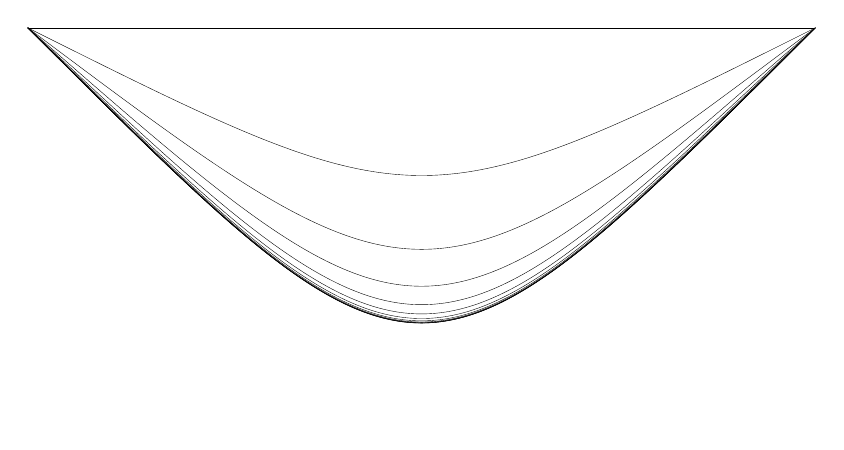
\begin{tikzpicture}[scale=5]
		\foreach \i in {0,1,2,...,12}{
			\draw[line width=0.05mm] (-1,1) .. controls (0,1/2^\i) .. (1,1);
		}
		\end{tikzpicture}
	\end{equation*}
\end{document}

A diagram to keep in mind
\begin{equation}
\begin{tikzcd}
\Z^{\infty} \arrow[r, "0"] & \Z^{\infty} \arrow[r, "1"] & \Z^{\infty} \arrow[r, "0"] & \Z^{\infty} \arrow[r, "1"] & \Z^{\infty} \\
\Z^{\infty} \arrow[r, "1"] \arrow[u, "0"] & \Z^{\infty} \arrow[r, "0"] \arrow[u, "0"] & \Z^{\infty} \arrow[r, "1"] \arrow[u, "1"] & \Z^{\infty} \arrow[r, "0"] \arrow[u, "0"] & \Z^{\infty} \arrow[u, "0"]
\end{tikzcd}
\end{equation}

Consider the following general diagram
\begin{equation}
\begin{tikzcd}
A_1 \arrow[r, "s_1"] & A_2 \arrow[r, "s_2"] & B \arrow[r, "t_1"] & C_1 \arrow[r, "t_2"] & C_2 \\
X_1 \arrow[r, "g_1"] \arrow[u, "0"] & X_2 \arrow[r, "g_2"] \arrow[u, "0"] & Y \arrow[r, "h_1"] \arrow[u, "f"] & Z_1 \arrow[r, "h_2"] \arrow[u, "0"] & Z_2 \arrow[u, "0"]
\end{tikzcd}
\end{equation}
